\documentclass{article}
\usepackage{../fasy-hw}
\usepackage{graphicx}

%% UPDATE these variables:
\renewcommand{\hwnum}{6}
\title{Advanced Algorithms, Homework \hwnum}
\author{Sarah Montalbano}
\collab{\todo{list your collaborators here}}
\date{due: Friday, 19 November 2021}

\begin{document}

\maketitle

This homework assignment should be
submitted as a single PDF file both to D2L and to Gradescope.

General homework expectations:
\begin{itemize}
    \item Homework should be typeset using LaTex.
    \item Answers should be in complete sentences and proofread.
    \item You will not plagiarize, nor will you share your written solutions
        with classmates.
    \item List collaborators at the start of each question using the
        \texttt{collab} command.
    \item Put your answers where the \texttt{todo} command currently is (and
        remove the \texttt{todo}, but not the word \texttt{Answer}).
    \item If you are asked to come up with an algorithm, you are
        expected to give an algorithm that beats the brute force (and, if possible, of
        optimal time complexity). With your algorithm, please provide the following:
        \begin{itemize}
            \item \emph{What}: A prose explanation of the problem and the algorithm,
                including a description of the input/output.
            \item \emph{How}: Describe how the algorithm works, including giving
                psuedocode for it.  Be sure to reference the pseudocode
                from within the prose explanation.
            \item \emph{How Fast}: Runtime, along with justification.  (Or, in the
                extreme, a proof of termination).
            \item \emph{Why}: Statement of the loop invariant for each loop, or
                recursion invariant for each recursive function.
        \end{itemize}
    \item The lowest HW grade is dropped.  However, this HW can only be dropped
        if the grade is at least 25\%.  (In other words, please do not choose to
        drop this homework by not doing any of it).
    \item This homework is an \textbf{individual} assignment.
\end{itemize}

\collab{None}
\nextprob{Describe an Algorithm}

Choose one concept or algorithm that you have learned
in this class so far. A student who has
taken 232 and 246, but not 432, has some questions about this problem:

\begin{enumerate}
    \item \emph{What} is the problem that this algorithm solves?

        \paragraph{Answer}
        Edit distance is the problem of quantifying the difference between two strings. Edit distance is calculated as the minimum number of letter insertions, letter deletions, and letter substitutions required to transform one string into another. The input to the edit distance algorithm is two strings $S_1$ and $S_2$ and the output is an integer representing the number of insertions, deletions, and substitutions required to transform one string into the other. If desired, tracing back through the saved answers to the subproblems of finding edit distance can yield the optimal alignment.

    \item \emph{How} does it work? (Describe in prose, with or without
        psuedocode.)

        \paragraph{Answer}        
The edit distance algorithm works on the principle that if we remove the last column, the remaining columns represent the shortest edit sequence for the remaining prefixes. For the last column, there are three possible choices the algorithm can make: an insertion, a deltion, or a substitution. In a recursive call, an insertion is $Edit(i, j-1) + 1$, where the + 1 represents the cost of making the insertion and the recursive call gives the minimum cost for the remaining alignment from $S_1[1..i]$ and $S_2[1..j-1]$. A deletion is $Edit(i - 1, j) + 1$, where the + 1 represents the cost of making the deletion and the recursive call gives the minimum cost for the remaining alignment from $S_1[1..i - 1]$ and $S_2[1..j]$. A substitution is $Edit(i - 1, j - 1) + 1$, where the + 1 represents the cost of making the substitution and the recursive call gives the minimum cost for the remaining alignment from $S_1[1..i - 1]$ and $S_2[1..j-1]$. (Note that the + 1 in each case may be replaced with some function that represents the different costs of insertions, deletions, and substitutions; for our purposes, we assume they are all penalized the same).

Our base cases occur where one or both strings are empty strings. Transforming the empty string into a string of length $j$ requires $j$ insertions. Similarly, transforming a string of length $i$ into an empty string requires $i$ deletions. Using a 2D array we can store the results of each recursive call so that the algorithm can reference it rather than calculating the same steps of the algorithm over and over again. The algorithm picks the minimum choice score of the insertion, deletion, and substitition options. 

\end{enumerate}


\collab{Weights on Vertices}
\nextprob{}

Chapter 8, Question 3, Part (a). Suppose we are given an undirected graph G in which every vertex has a positive weight. Describe and analyze an algorithm to find a spanning tree of G with minimum total weight. (The total weight of a spanning tree is the sum
of the weights of its vertices.)

\paragraph{Answer}
\todo{TODO}
\begin{itemize}
            \item \emph{What}: 
A prose explanation of the problem and the algorithm,
                including a description of the input/output.
            \item \emph{How}: Describe how the algorithm works, including giving
                psuedocode for it.  Be sure to reference the pseudocode
                from within the prose explanation.
            \item \emph{How Fast}: Runtime, along with justification.  (Or, in the
                extreme, a proof of termination).
            \item \emph{Why}: Statement of the loop invariant for each loop, or
                recursion invariant for each recursive function.
        \end{itemize}

\nextprob{MED}
Consider the randomized minimum enclosing disc (MED) algorithm.  In this
homework, we investigate the worst-case analysis of it.  In class, we will study
the randomized analysis.

\begin{algorithm}\caption{\textsc{MED($S$, $\Sigma$)}}\label{alg:seb}
    {\bf Input:} two finite sets $S$, $\Sigma \subset \R^2$\\
    {\bf Output:} $B$, the smallest ball enclosing $S$ with points of
    $\Sigma$ on the boundary.

    \begin{algorithmic}[1]
        \If{$|S|=0$}\\
        ~~~~~~\Return the smallest ball with $\Sigma$ on boundary
        \EndIf

        \State $i \gets \textsc{Random}(n)$
        \State $B = \textsc{MED}(S \backslash S[i], \Sigma)$
        \If{$S[i] \in B$}\\
        ~~~~~~\Return $B$
        \Else\\
        ~~~~~~\Return $\textsc{MED}\left((S \backslash S[i], \Sigma \cup \{ S[i]
        \}\right)$
        \EndIf
    \end{algorithmic}
\end{algorithm}

In the above algorithm, suppose $\textsc{Random}(n)$ returns a random integer
between $1$ and $n$ (inclusive).  Further suppose
$S$ is stored as an array with indices $1$ though $n$,
and $|\Sigma| \leq 3$.  Let's represent the output ball as an ordered
pair~$B=(b_c,b_r) \in \R^2 \times \R_{\geq 0}$,
where $b_c\in \R^2$ is the center of a smallest enclosing ball and $b_r$ is the
radius of the smallest enclosing ball.

\begin{enumerate}[(a)]
    \item
        Suppose $S=\emptyset$ and $\Sigma=\{ (a_x,a_y)\}$. What ball is returned on Line 2?
        \paragraph{Answer}
        \todo{answer here}
    \item
        Suppose $S=\emptyset$ and $\Sigma=\{ a=(a_x,a_y),b=(b_x,b_y)\}$, what ball is returned on Line 2?
        \paragraph{Answer}
        \todo{answer here}
    \item
        Suppose $S=\emptyset$ and $\Sigma=\{ a=(a_x,a_y),b=(b_x,b_y)\}$, what ball is returned on Line 2?
        \paragraph{Answer}
        \todo{answer here}

    \item Let $T(n)$ be the time complexity of MED($S$, $\Sigma$) when
        $|S|=n$.  Give the worst-case recurrence~relation.
        \paragraph{Answer}
        \todo{answer here}
    \item What is the closed form of your answer to (c)?
        \paragraph{Answer}
        \todo{answer here}
\end{enumerate}


\collab{None
}
\nextprob{Algorithms in the News}

Find an algorithm discussed in a recent news article (over the past 12 months).
Choose ONE of the following:
\begin{enumerate}
    \item Look up the primary resource for this algorithm (likely to be a
        research paper).  Compare/contrast the similarities and differences between the
        way the news article describes the problem and algorithm with the way
        that the primary resource describes it.
    \item If the algorithm itself is not given in the article, provide a prose
        description of the algorithm along with pseudocode. (This might require
        looking up the primary resource for the algorithm).
    \item Analyze the runtime of the algorithm.
    \item Prove the correctness of the algorithm.
\end{enumerate}

\paragraph{Answer}
\todo{answer here}
\url{https://www.wired.com/story/computer-scientists-find-a-key-research-algorithms-limits/}

\collab{TODO}
\nextprob{Decrementing Function}

Prove that the generic algorithm for SSSP, \textsc{FordSSSP}, terminates using a
decrementing function.

\paragraph{Answer}
\todo{answer here}

\collab{TODO}
\nextprob{All Pairs Shortest Paths}

Walk through \textsc{ShimbelAPSP} algorithm (Erickson, page 314) for the graph given in class on
11/10/21.

\paragraph{Answer}
\todo{answer here}
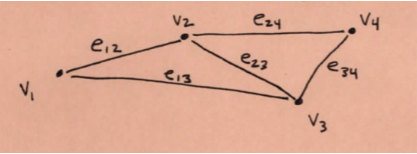
\includegraphics{graph.png}




\end{document}
